\documentclass[11pt, oneside]{article} 
\usepackage{geometry}
\geometry{letterpaper} 
\usepackage{graphicx}
	
\usepackage{amssymb}
\usepackage{amsmath}
\usepackage{parskip}
\usepackage{color}
\usepackage{hyperref}

\graphicspath{{/Users/telliott_admin/Dropbox/Tex/png/}}
% \begin{center} \includegraphics [scale=0.4] {gauss3.png} \end{center}

\title{Area}
\date{}

\begin{document}
\maketitle
\Large

I became aware later that there is yet another way to apply the method, and that is to calculate the \emph{areas} of inscribed and circumscribed polygons.  We'll go through this briefly.

For this approach we use a unit circle (radius $1$) rather than a diameter of $1$, as we did above.  As before, we define $\theta$ to be the central angle of the half-sector (i.e. $\theta = 2\pi/2n$).
\begin{center} 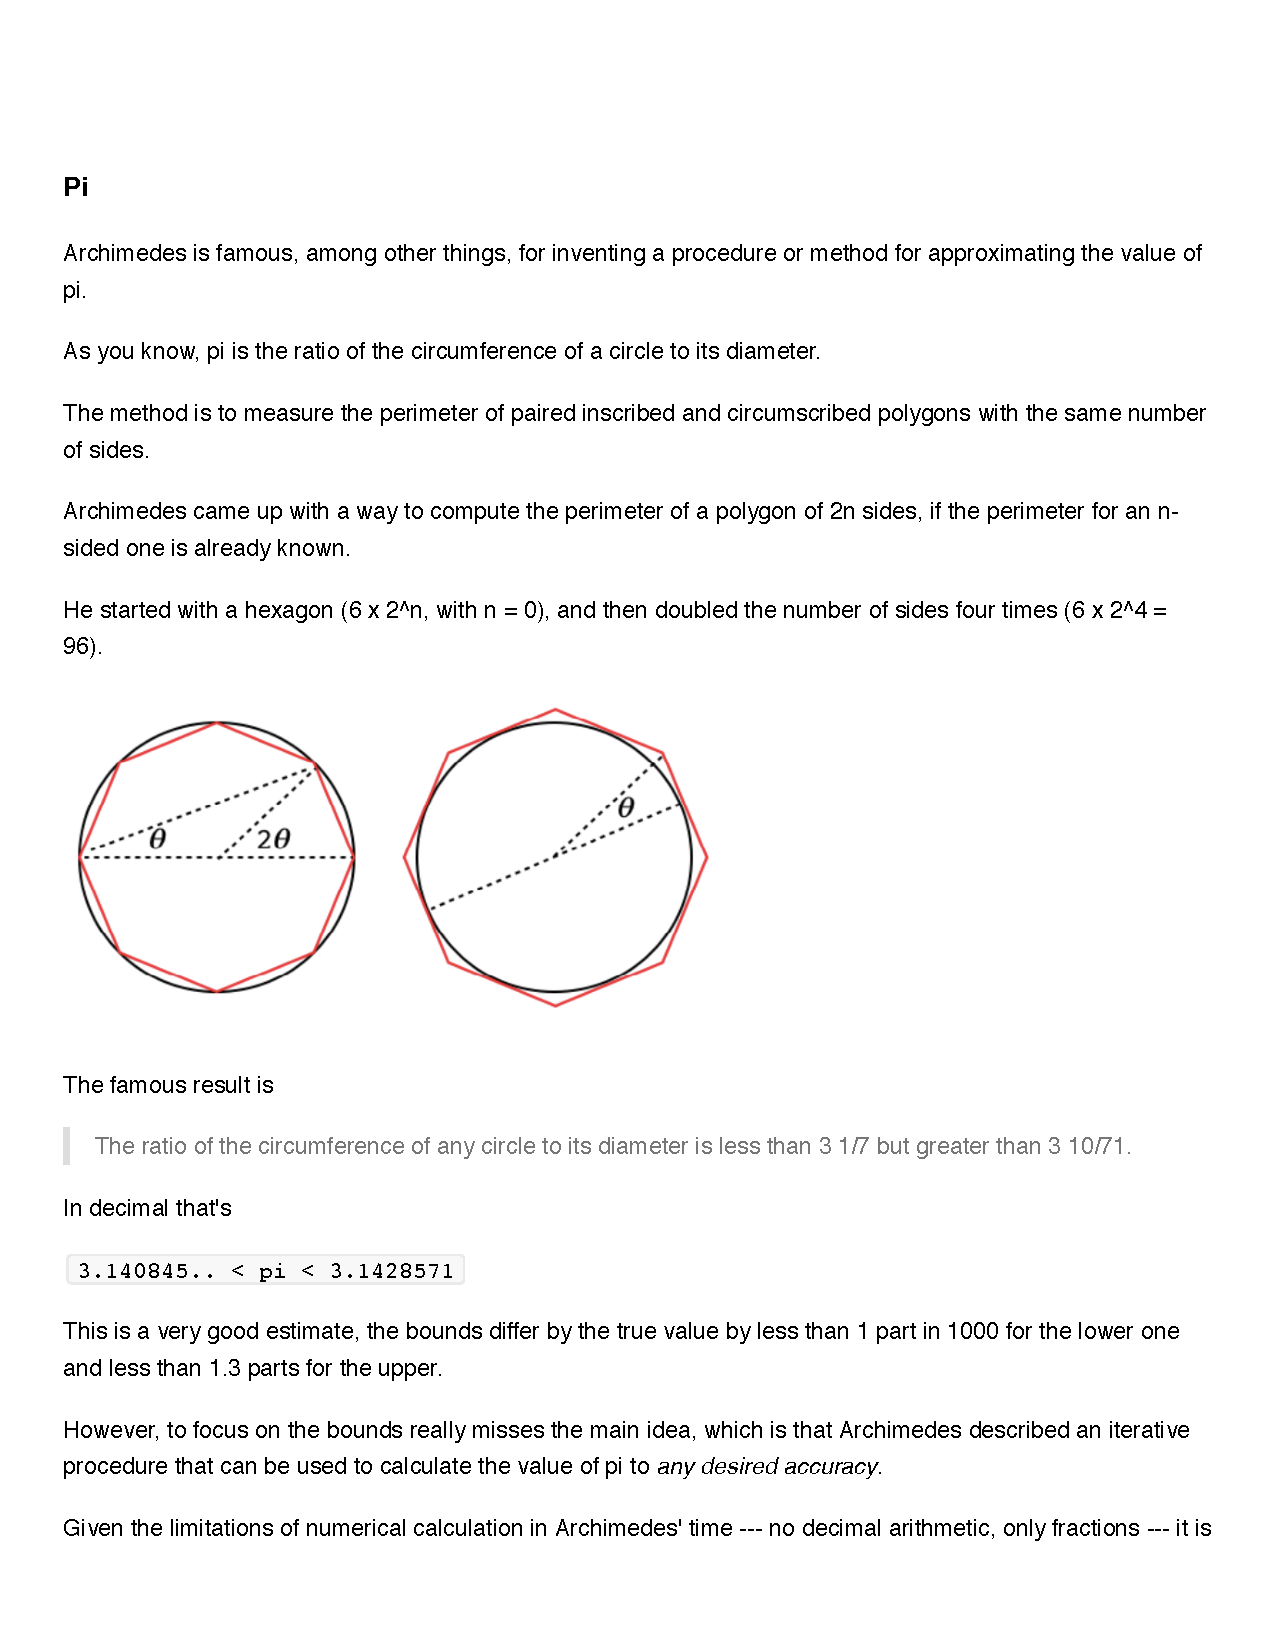
\includegraphics [scale=0.5] {pi.png} \end{center}
Rather than draw an entirely new figure, just imagine in the left panel that we draw the angle bisector of angle $2 \theta$.  The area of each new triangle is then $\sin \theta \cos \theta / 2$ and the total area of the inner polygon is
\[ a = n \sin \theta \cos \theta = n SC \]
in the notation we adopted previously in this chapter.  And, as before, to progress to $a'$ we have a factor of $2$ as well as the new values $S'$ and $C'$:
\[ a' = 2n S'C' \]

For the circumscribed or outer polygon, we just have what we had before, that the side length of the triangle in the right panel is $\tan \theta$ so the total area is
\[ A = nT \]

Bring in the half-angle formulas as follows:
\[ a' = 2n S'C' = 2n \cdot \frac{S}{2C'} \cdot C' = nS \]
That is slick, but we need an expression for $nS$:
\[ aA = nSC \cdot n \frac{S}{C} = [nS]^2 \]
\[ aA = [a']^2 \]
\[ a' = \sqrt{aA} \]

This is like, and yet subtly different than what we had when calculating the perimeter.

Since
\[ A = nT \]
and
\[ A' = 2nT' \]
\[ = 2n \frac{ST}{S + T} = 2 \frac{nS \cdot nT}{nS + nT} \]
\[ A' = 2 \frac{a'A}{a' + A} \]
Compare
\[ a' = \sqrt{aA}  \ \ \ \ \  A' = 2 \frac{a'A}{a' + A} \]
\[ p' = \sqrt{pP'}  \ \ \ \ \   P' = 2 \frac{pP}{p + P} \]

\end{document}